\section{Die Elementaren Tools}
\begin{frame}
    \Huge
    \centering
    Legt euch ein System für Notizen zu!

\end{frame}

\begin{frame}{Anforderungen}
    \begin{columns}[t]
        \begin{column}[t]{0.15\textwidth}
            \begin{tikzpicture}
                %\useasboundingbox[fill=red] (0,0) rectangle(0.3*\paperwidth,\the\paperheight);
                \node[anchor=north west] at (0.3cm,6cm) {
\includegraphics[height=1.6cm]{graphics/F.pdf}};
                \node[anchor=north west] at (0cm,4cm) {
\includegraphics[height=1.6cm]{graphics/A.pdf}};
                \node[anchor=north west] at (0.5cm,2cm) {
\includegraphics[height=1.6cm]{graphics/I.pdf}};
                \node[anchor=north west] at (0.3cm,0cm) {
\includegraphics[height=1.6cm]{graphics/R.pdf}};
            \end{tikzpicture}
        \end{column}
        \begin{column}[t]{0.84\textwidth}
            \vspace{-8cm}
            \begin{itemize}
                \setlength{\itemindent}{-2em}
                \item[] \textbf{F}indable - Auffindbar
                \begin{itemize}
                    \item Eure Daten sollten leicht zu durchsuchen sein
                    \item Eure Daten sollten gut strukturiert sein
                \end{itemize}
                \item[] \textbf{A}ccessible - Zugänglich
                \begin{itemize}
                    \item Ihr solltet jederzeit Zugang zu euren Daten haben
                    \begin{itemize}
                        \item Habt immer eine lokale Kopie!
                    \end{itemize}
                \item Macht eure Notizen auch euren Komilitonen zugänglich
            \end{itemize}
                \item[] \textbf{I}nteroperable - Interoperabel
                \begin{itemize}
                    \item Verwendet gängige Dateiformate
                    \item Stellt eure Quellen offen, nicht nur PDFs
                    \item Sucht euch Tools die ihr verbinden könnt
                \end{itemize}
                \item[] \textbf{R}eusable - Wiederverwendbar
                \begin{itemize}
                    \item Übersetzt eure Unterlagen in wieder nutzbares Wissen
                \end{itemize}
            \end{itemize}
        \end{column}
    \end{columns}  
\end{frame}

\begin{frame}{Aber welches? Die einfache Antwort zuerst} 
    \begin{tikzpicture}
        \node[anchor=south west] at (0,2) {
\includegraphics[width=3cm]{graphics/Logos/GoogleWorkspace.jpeg}};
        \node[anchor=south west] at (3,1) {
\includegraphics[width=3cm]{graphics/Logos/Office365.png}};
        \node[anchor=south west] at (6,3) {
\includegraphics[width=3cm]{graphics/Logos/Evernote.jpeg}};
        \node[anchor=south west] at (9,2) {
\includegraphics[width=3cm]{graphics/Logos/Notion.jpeg}};
    \end{tikzpicture}
    \pause\\
    \centering\large Es muss zu eurem Stil passen!    

\end{frame}
\note{Search, Cloud, Collab, Meetings, Local, conversion\\}

\begin{frame}[t]{Cloud}
    \begin{columns}[t]   
        \begin{column}{0.29\textwidth}      
            \vspace{-3em}      
            \begin{figure}[t]
                \begin{flushleft}
                    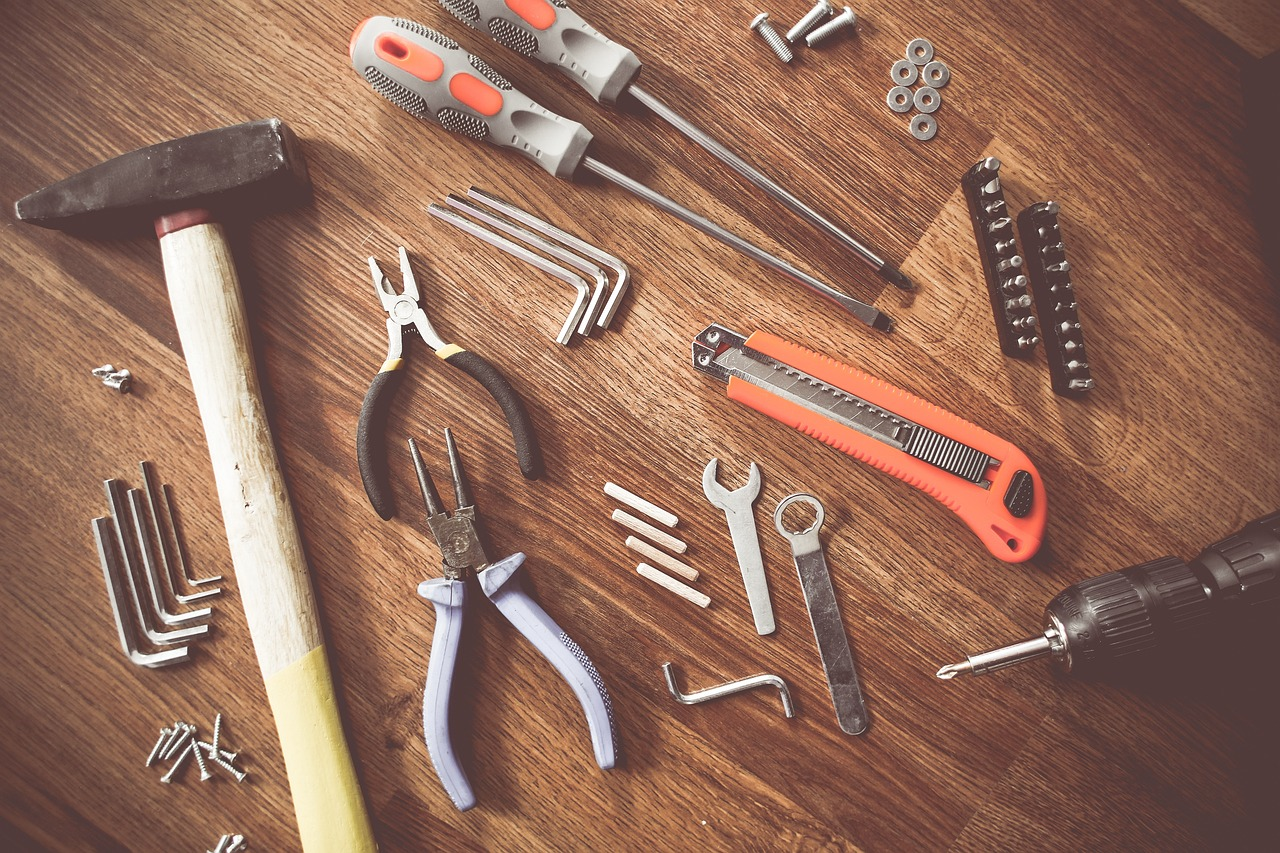
\includegraphics[height=0.8\textheight,trim={0 0 25cm 0},clip]{graphics/tools-864983_1280.jpg}         
                    \caption*{\href{https://pixabay.com/de/photos/werkzeuge-konstruieren-boot-864983/}{picjumbo\_com on pixabay}}    
                \end{flushleft}                
            \end{figure}
        \end{column} 
        \begin{column}{0.7\textwidth}
            Warum?
            \begin{itemize}[]
                \item Macht eure Daten überall Verfügbar
                \item Erlaubt einfaches Teilen von Daten
            \end{itemize}
            Welche?
            \begin{itemize}[]
                \item Dropbox, Google Cloud, iCloud
                \item Sciebo
                \begin{itemize}
                    \item Sciebo: Die Hochschulcloud verfügbar an allen Deutschen Hochschulen
                    \item Hostet in Deutschland
                    \item Kostenlose 30 GB
                \end{itemize}
            \end{itemize}
            Kriterien?
            \begin{itemize}[]
                \item $\geq$ 15 GB Speicherplatz
                \item Kostenlos
            \end{itemize}
        \end{column}        
    \end{columns}
\end{frame}

\begin{frame}[t]{Notizen}
    \begin{columns}[t]
        \begin{column}{0.29\textwidth}      
            \vspace{-3em} 
            \begin{figure}[t]
                \begin{flushleft}
                    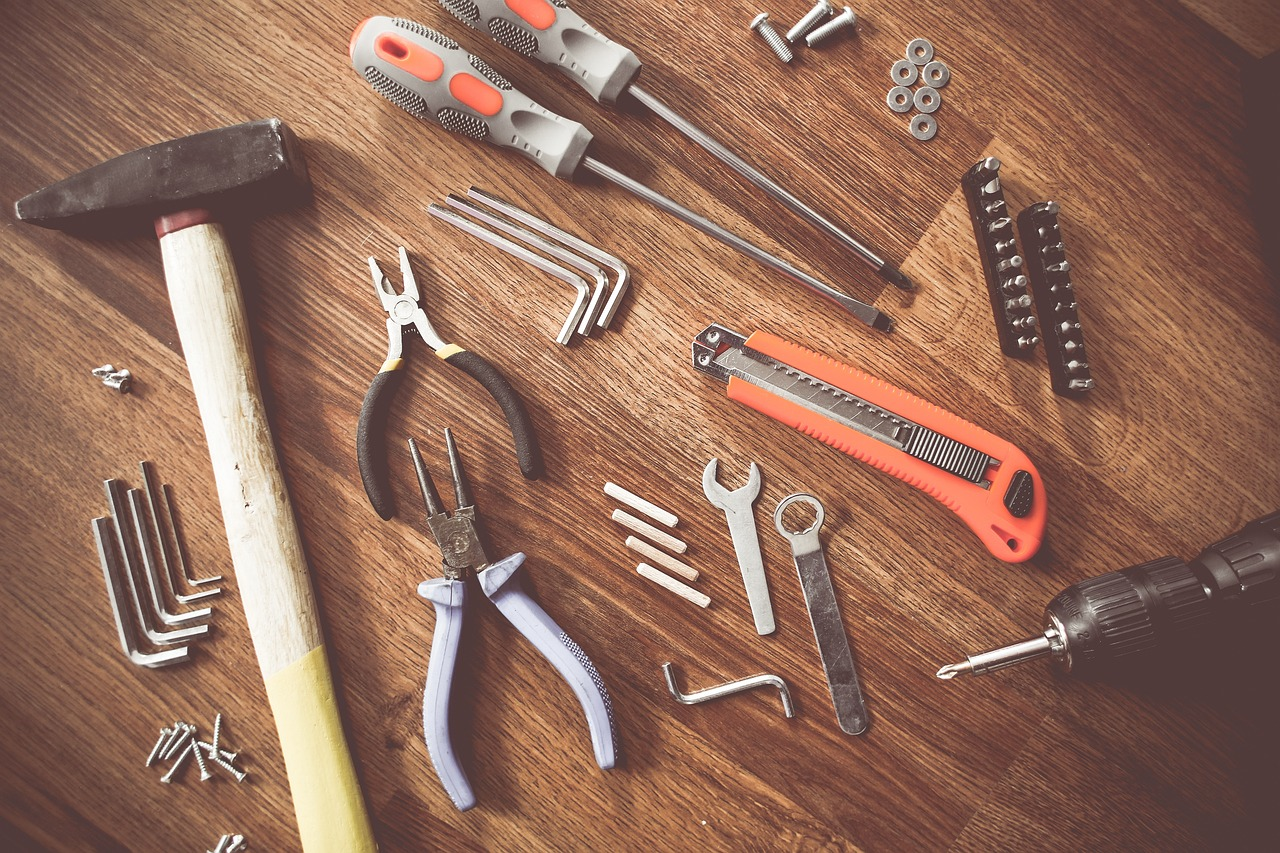
\includegraphics[height=0.8\textheight,trim={0 0 25cm 0},clip]{graphics/tools-864983_1280.jpg}         
                    \caption*{\href{https://pixabay.com/de/photos/werkzeuge-konstruieren-boot-864983/}{picjumbo\_com on pixabay}}    
                \end{flushleft}                
                      
            \end{figure}
        \end{column}        
        \begin{column}{0.7\textwidth}
            Welche?
            \begin{itemize}[]
                \item Google Docs, MS Word, Libre Office
                \item OneNote, Notion
                \item Obsidian, Joplin
            \end{itemize}
            Kriterien?
            \begin{itemize}[]
                \item Verfügbar auf allen Geräten
                \item Dateien übergreifende Suche
                \item Notizen Verknüpfen von Dateien
                \item Verknüpfungen zu Quellen herstellen
            \end{itemize}
        \end{column}
    \end{columns}
\end{frame}

\note{Ihr werdet immer eine Software brauchen, in der ihr Notizen anlegen könnt.
Word ist ein klassiker, aber nicht optimal für notizen.
OneNote ist ebenfalls von Microsoft, ist sehr flexibel, aber verwendet kein gängiges Format.
Joplin und Obsidian sind beides Tools die auf Markdown basieren.
Zusätzlich zu Notizen, müsst ihr die natürlich auch irgendwo Speichern, zusammen mit euren anderen Materialien.
Eine Cloud Lösung ist dafür ideal.
Dropbox ist eine der älteren und verbreiteten Lösungen. Sciebo ist eine alternative die von fast allen Universitäten angeboten wird. 
}



\subsection{Literatur}

\begin{frame}{Literatur Verwaltung}
    \begin{columns}[t]
        \begin{column}{0.39\textwidth}      
            \vspace{-2em} 
            \begin{figure}[t]
                \begin{flushleft}
                    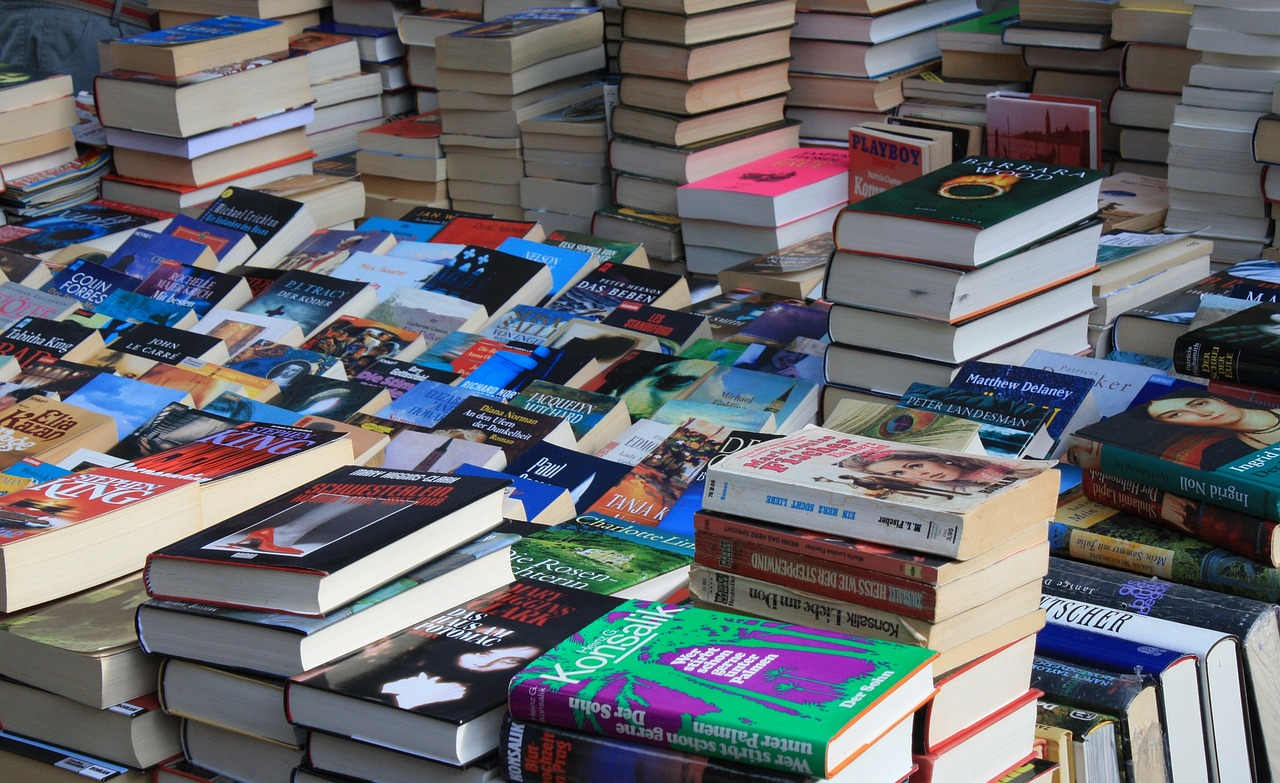
\includegraphics[height=0.8\textheight,trim={11cm 0 15cm 0},clip]{graphics/Flohmarkt.jpg}         
                    \caption*{\href{https://pixabay.com/de/photos/flohmarkt-bücher-kiste-stöbern-237460/}{geralt on pixabay}}    
                \end{flushleft}
            \end{figure}
        \end{column}          
        \begin{column}{0.69\textwidth}
            \begin{itemize}
                \item Citavi
                \item Mendeley
                \item Zotero
                \pause
                \begin{itemize}
                    \item Open Source
                    \item Kostenlos
                    \item Kompatibel mit MS Office, Google Docs and LaTeX
                    \item Features für PDF Annotation, Markieren und Notizen
                \end{itemize}
            \end{itemize}           
        \end{column}        
    \end{columns}    
\end{frame}

\begin{frame}{Literatur Recherche}
    \begin{columns}[t]
        \begin{column}{0.39\textwidth}      
            \vspace{-2em} 
            \begin{figure}[t]
                \begin{flushleft}
                    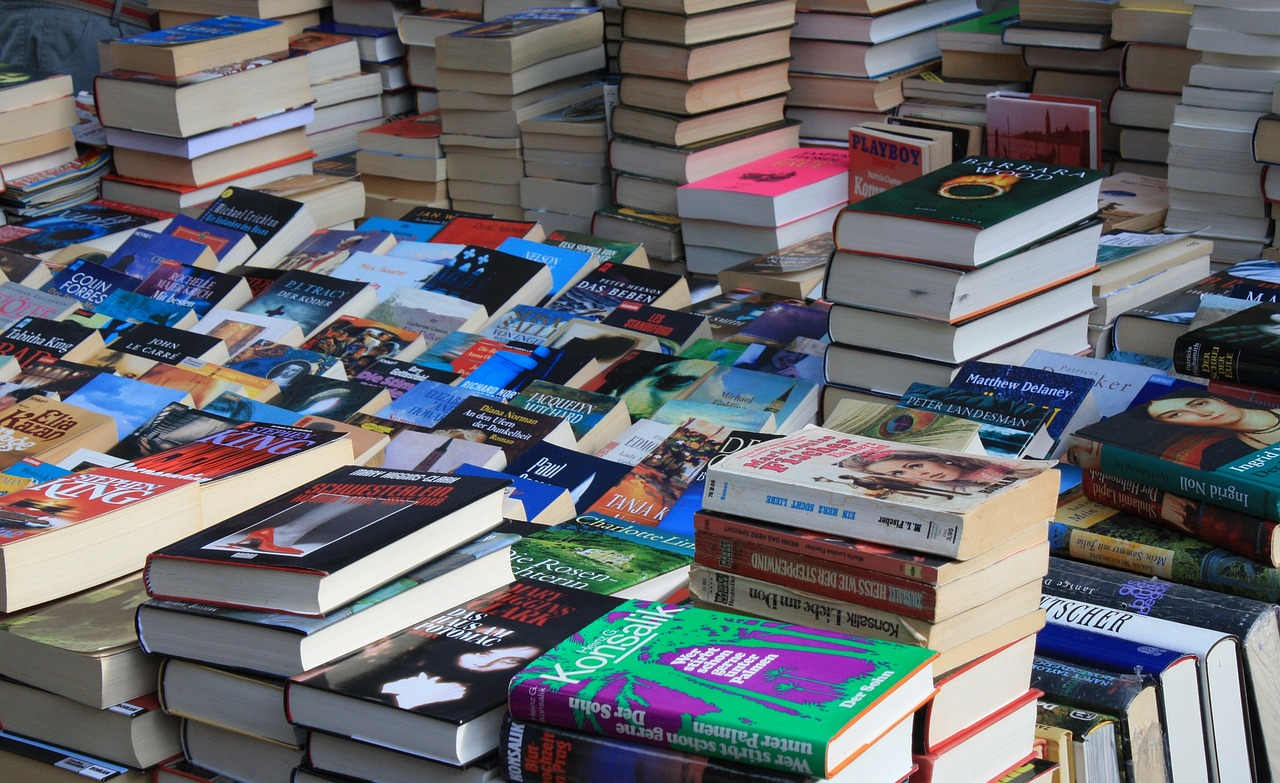
\includegraphics[height=0.8\textheight,trim={11cm 0 15cm 0},clip]{graphics/Flohmarkt.jpg}         
                    \caption*{\href{https://pixabay.com/de/photos/flohmarkt-bücher-kiste-stöbern-237460/}{geralt on pixabay}}    
                \end{flushleft}
            \end{figure}
        \end{column}        
        \begin{column}{0.69\textwidth}
            \begin{itemize}
                \item Google, \href{https://scholar.google.com/}{Google Scholar}
                \item \href{https://www.connectedpapers.com/}{Connected Papers}
                \item \href{https://elicit.com/}{Elicit}
                \item ChatGPT
                \item Eure Uni Bibliothek!
            \end{itemize}           
            \vspace{1cm}            
            \begin{itemize}
                \item \textcolor{lightgray}{libgen.ist}
                \item \textcolor{lightgray}{scihub.st}
            \end{itemize} 
        \end{column}        
    \end{columns}  
\end{frame}

\begin{frame}{Andere Materialien}
    \begin{columns}[t]
        \begin{column}{0.39\textwidth}      
            \vspace{-2em} 
            \begin{figure}[t]
                \begin{flushleft}
                    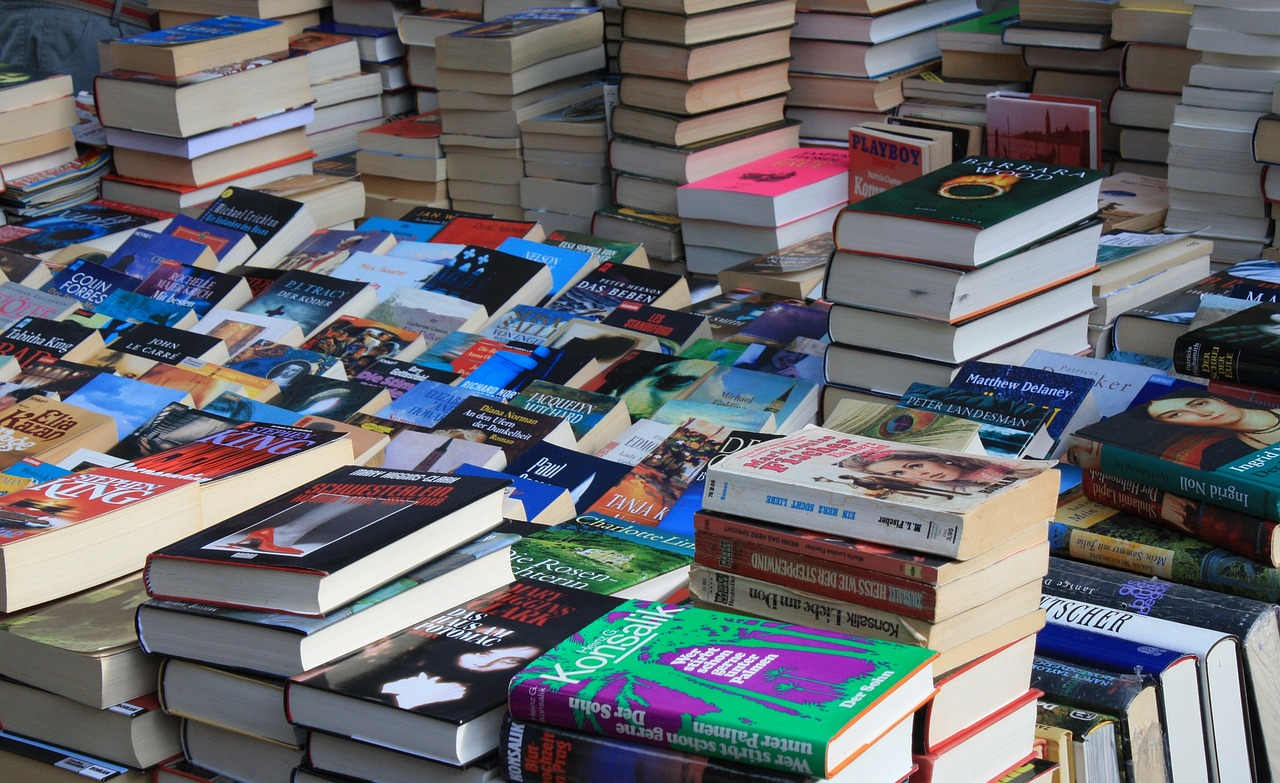
\includegraphics[height=0.8\textheight,trim={11cm 0 15cm 0},clip]{graphics/Flohmarkt.jpg}         
                    \caption*{\href{https://pixabay.com/de/photos/flohmarkt-bücher-kiste-stöbern-237460/}{geralt on pixabay}}    
                \end{flushleft}
            \end{figure}
        \end{column}          
        \begin{column}{0.69\textwidth}
            \begin{itemize}
                \item Hörbücher
                \begin{itemize}
                    \item LibriVox, Audible 
                \end{itemize}
                \item Bilder \& Grafiken
                \begin{itemize}
                    \item Google Bilder, Pixabax, Pexels
                \end{itemize}
                \item Vorlagen
                \begin{itemize}
                    \item Powerpoint: AllPPT.com
                    \item \LaTeX: Overleaf.com
                \end{itemize}

            \end{itemize}           
        \end{column}        
    \end{columns}    
\end{frame}

\begin{frame}[t]{Schreiben}
    \begin{columns}[t]
        \begin{column}{0.29\textwidth}      
            \vspace{-3em} 
            \begin{figure}[t]
                \begin{flushleft}
                    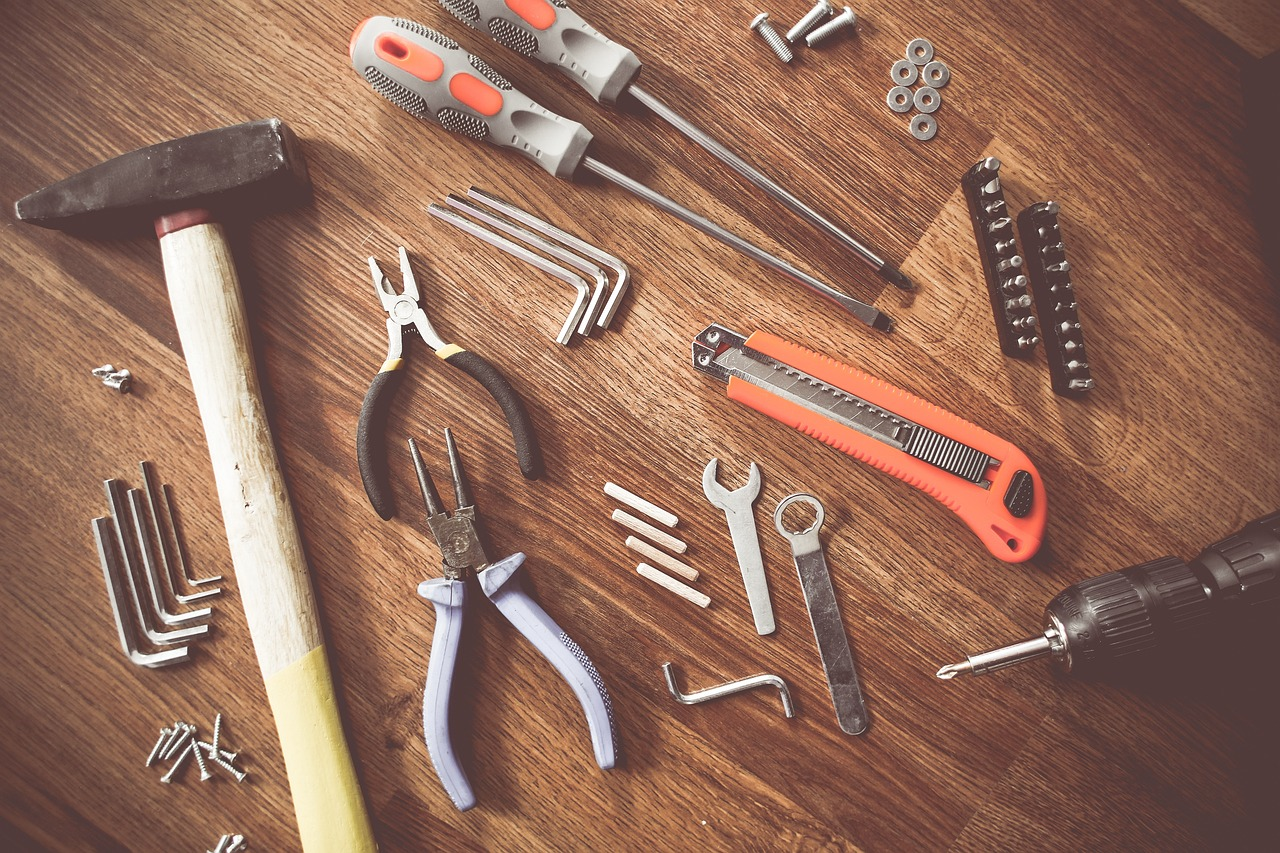
\includegraphics[height=0.8\textheight,trim={0 0 25cm 0},clip]{graphics/tools-864983_1280.jpg}         
                    \caption*{\href{https://pixabay.com/de/photos/werkzeuge-konstruieren-boot-864983/}{picjumbo\_com on pixabay}}    
                \end{flushleft}                
                      
            \end{figure}
        \end{column}        
        \begin{column}{0.7\textwidth}
            Welche?
            \begin{itemize}[]
                \item Google Docs, MS Word, Libre Office Write
                \item \LaTeX
                \item Markdown
            \end{itemize}
            Kriterien?
            \begin{itemize}[]
                \item Hochwertiger Output
                \item Einfaches Refferenzieren von Quellen
                \item Automatische Inhaltverzeichnisse
            \end{itemize}
        \end{column}
    \end{columns}
\end{frame}

\begin{frame}[t]{Präsentieren}
    \begin{columns}[t]
        \begin{column}{0.29\textwidth}      
            \vspace{-3em} 
            \begin{figure}[t]
                \begin{flushleft}
                    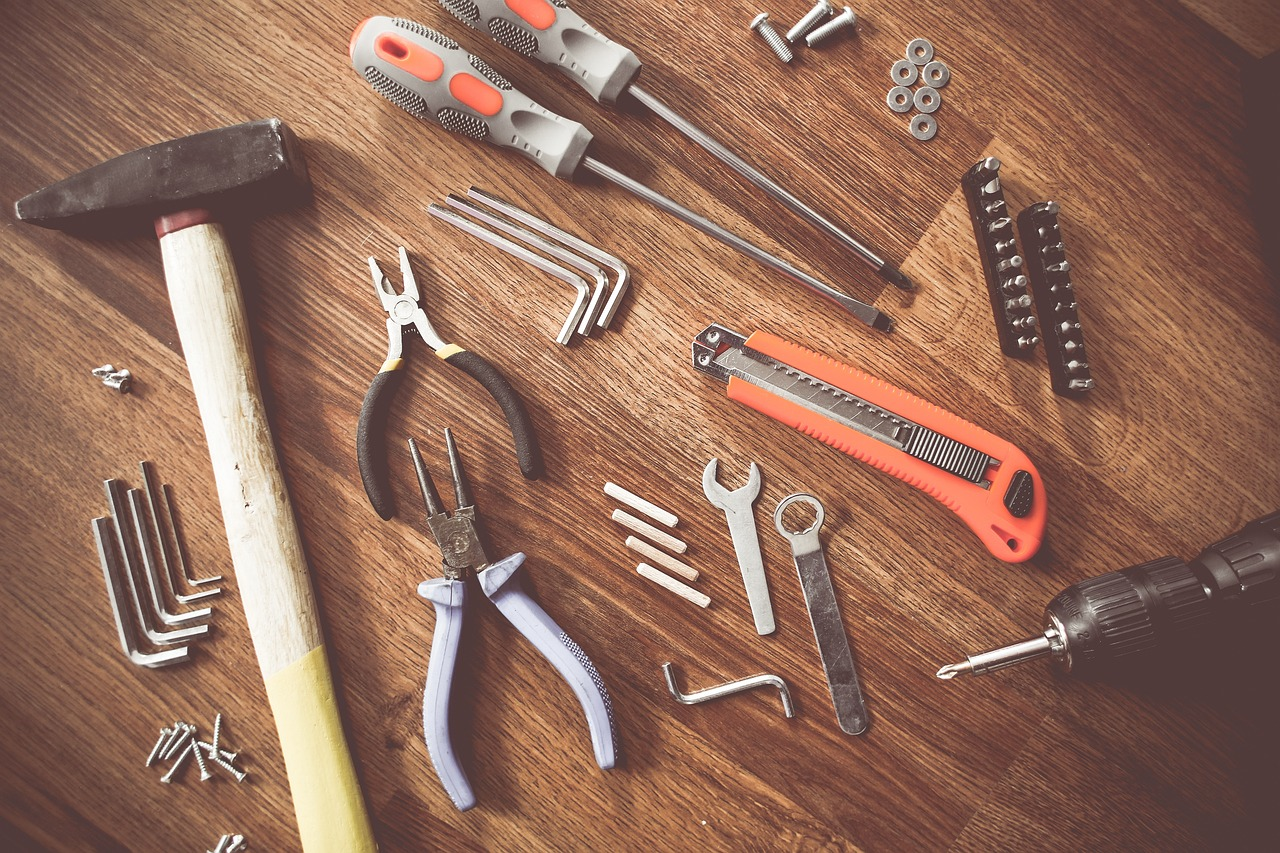
\includegraphics[height=0.8\textheight,trim={0 0 25cm 0},clip]{graphics/tools-864983_1280.jpg}         
                    \caption*{\href{https://pixabay.com/de/photos/werkzeuge-konstruieren-boot-864983/}{picjumbo\_com on pixabay}}    
                \end{flushleft}                
                      
            \end{figure}
        \end{column}        
        \begin{column}{0.7\textwidth}
            Welche?
            \begin{itemize}[]
                \item Google Slides, PowerPoint LibreOffice Präsentationen
                \item \LaTeX
                \item Markdown
            \end{itemize}
            Kriterien?
            \begin{itemize}[]
                \item Hochwertiger Output
            \end{itemize}
        \end{column}
    \end{columns}
\end{frame}

\begin{frame}{Rechtschreibung und Gramatik}
    \begin{columns}[t]
        \begin{column}{0.4\textwidth}
            \vspace{-2em} 
            \begin{figure}
                \begin{flushleft}
                    
\includegraphics[height=0.6\textheight,trim={8cm 10 2cm 0},clip]{graphics/correcting-1870721_1280.jpg}
                    \caption*{\href{https://pixabay.com/photos/correcting-proof-paper-correction-1870721/}{3844328 on pixabay}}    
                \end{flushleft}                
            \end{figure}
            
        \end{column}
        \begin{column}{0.6\textwidth}
            \begin{itemize}
                \item Gramarly
                \item DudenMentor
                \item LanguageTool
                \begin{itemize}
                    \item Plugins für gängige Browser
                    \item Auch in der freien Version sehr Mächtig
                \end{itemize}
            \end{itemize}
        \end{column}
    \end{columns}
\end{frame}

\begin{frame}[t]{Mein Tipp: Text Dateien}
    \begin{columns}[t]
        \begin{column}{0.29\textwidth}      
            \vspace{-3em} 
            \begin{figure}[t]
                \begin{flushleft}
                    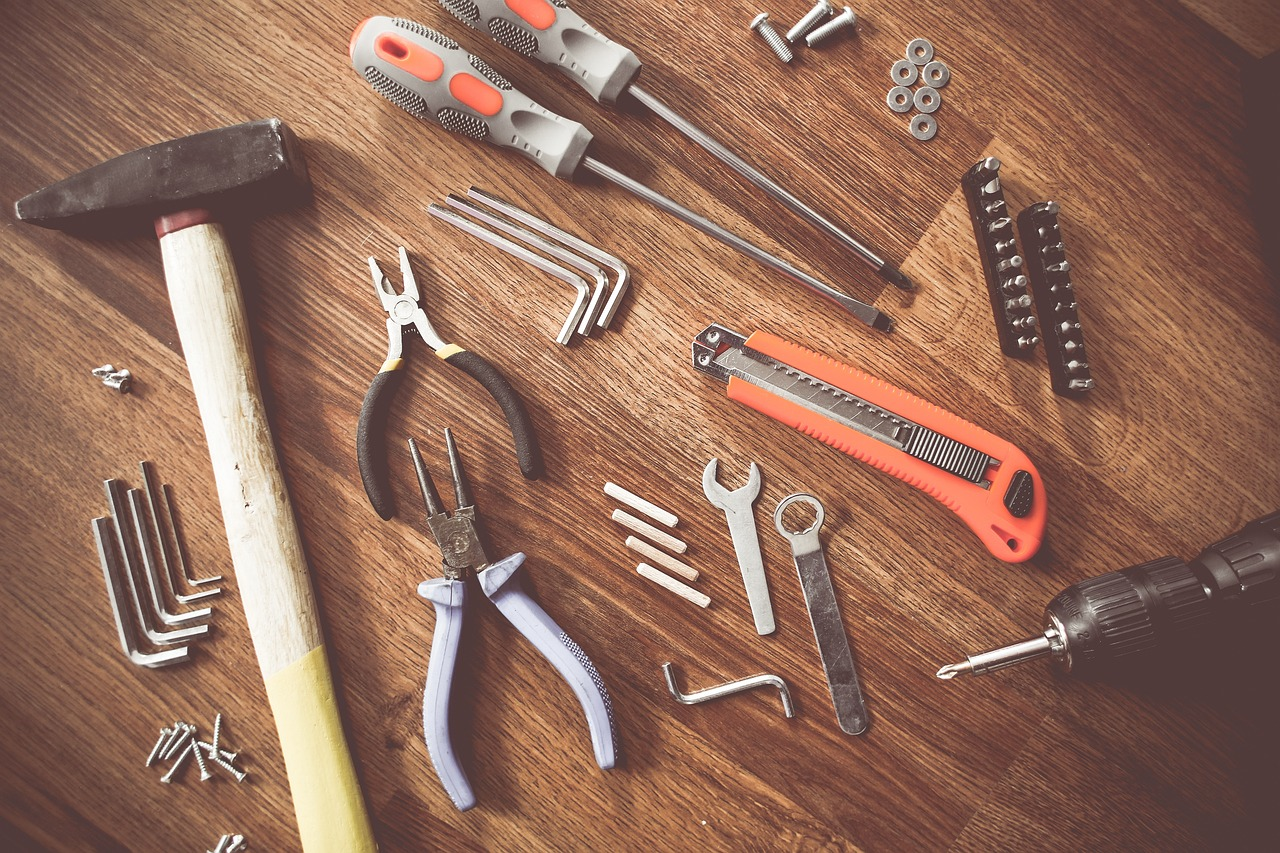
\includegraphics[height=0.8\textheight,trim={0 0 25cm 0},clip]{graphics/tools-864983_1280.jpg}         
                    \caption*{\href{https://pixabay.com/de/photos/werkzeuge-konstruieren-boot-864983/}{picjumbo\_com on pixabay}}    
                \end{flushleft}                
                      
            \end{figure}
        \end{column}        
        \begin{column}{0.7\textwidth}
            Plain Text
            \begin{itemize}
                \item ist portabel
                \item ist kompakt
                \item ist leicht zu durchsuchen
                \item einfach zu verwalten
            \end{itemize}
        \end{column}
    \end{columns}
\end{frame}


\begin{frame}{GIT}
    \begin{columns}
        \begin{column}{0.4\textwidth}
            \begin{flushleft}
                \begin{figure}
                    
\includegraphics[height=0.8\textheight]{graphics/final.jpg}
                \end{figure}    
            \end{flushleft}            
        \end{column}
        \begin{column}[t]{0.6\textwidth}
            \pause
            \vspace{-4cm}
            \begin{itemize}[]
                \item GIT
                \begin{itemize}
                    \item Erlaubt inkrementelles Verändern von Dateien
                    \item Gibt euch eine Historie aller Änderugen
                    \item und eine Zeitmaschiene
                \end{itemize}
                \item Aber hat eine steile Lernkurve
            \end{itemize}
            
        \end{column}
    \end{columns}
\end{frame}
